\subsection{Esercizio 25}
Utilizzare le formule tabulate nel precedente esercizio per calcolare le approssimazioni dell'integrale
\[
    I(f) = \int_{0}^{1} e^{3x}\,dx,
\]
tabulando (in modo significativo) il corrispondente errore di quadratura (risolvere a mano l'integrale).
\newline \textbf{Soluzione:}

Eseguendo lo script \nameref{cod:25} si ottengono i risultati contenuti nella tabella \ref{tab:25}
e nella figura \ref{fig:es25}.
\begin{table}[ht]
    \centering
    \renewcommand\arraystretch{2}
    \begin{tabular}{| c | c |}
        \hline
        n & $E_n(f)$              \\
        \hline
        1 & 4.180922820531277e+00 \\
        2 & 1.402032263607644e-01 \\
        3 & 6.409819710703601e-02 \\
        4 & 1.827410064641377e-03 \\
        5 & 1.038246005102827e-03 \\
        6 & 1.990061006917898e-05 \\
        7 & 1.226107634089146e-05 \\
        9 & 1.049225657467900e-07 \\
        \hline
    \end{tabular}
    \caption{Errori di quadratura per $I(f)$}
    \label{tab:25}
\end{table}
\FloatBarrier
\begin{figure}[!ht]
    \centering
    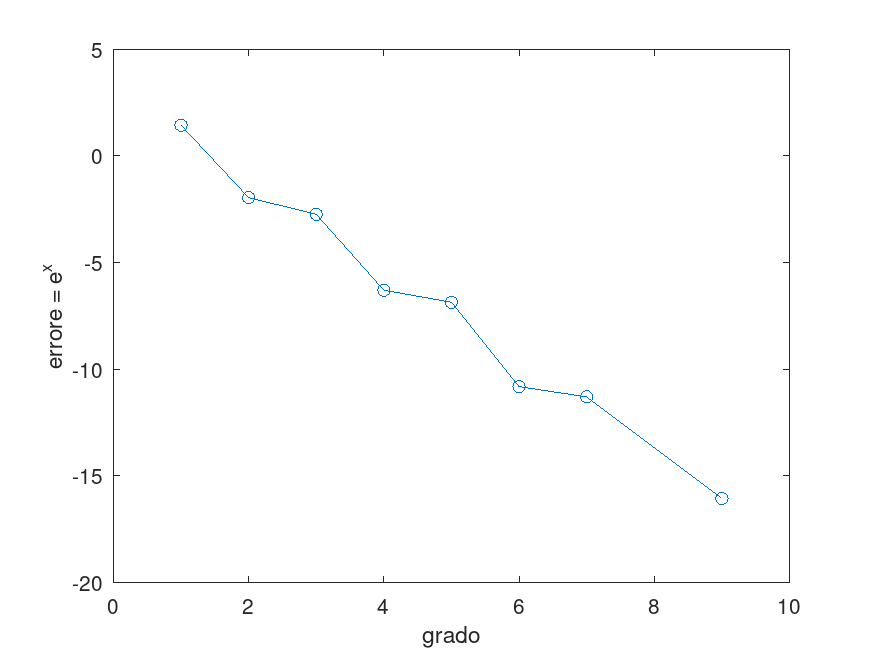
\includegraphics[width=16cm,height=10cm,keepaspectratio]{capitolo5/es25_figure.png}
    \caption{Errori di quadratura rispetto a grado per $I(f)$}
    \label{fig:es25}
\end{figure}
\FloatBarrier
